%% LyX 2.0.5.1 created this file.  For more info, see http://www.lyx.org/.
%% Do not edit unless you really know what you are doing.
\documentclass[english,letterpaper, 10 pt, conference]{ieeeconf}
\IEEEoverridecommandlockouts                              % This command is only
\overrideIEEEmargins

\let\proof\relax 
\let\endproof\relax
\usepackage{mathpazo}
\usepackage[T1]{fontenc}
\usepackage[latin9]{inputenc}
\usepackage{array}
\usepackage{prettyref}
\usepackage{float}
\usepackage{textcomp}
\usepackage{multirow}
\usepackage{amsthm}
\usepackage{amsmath}
\usepackage{amssymb}
\usepackage{graphicx}

\makeatletter

%%%%%%%%%%%%%%%%%%%%%%%%%%%%%% LyX specific LaTeX commands.
%% Because html converters don't know tabularnewline
\providecommand{\tabularnewline}{\\}

%%%%%%%%%%%%%%%%%%%%%%%%%%%%%% Textclass specific LaTeX commands.
\numberwithin{equation}{section}
\numberwithin{figure}{section}

\@ifundefined{date}{}{\date{}}
%%%%%%%%%%%%%%%%%%%%%%%%%%%%%% User specified LaTeX commands.
\IEEEoverridecommandlockouts
\overrideIEEEmargins
\usepackage{fixltx2e}
\usepackage{hyperref}

% add [table] to allow \rowcolor
\usepackage[table]{xcolor} 

\newcommand{\mythanks}{\thanks{A.\ Censi is with the Computing \& Mathematical Sciences department, Division of Engineering and Applied Sciences, California Institute of Technology, Pasadena, CA. E-mail: andrea@cds.caltech.edu. 
J.\ Strubel and D.\ Scaramuzza are with Department of Informatics, University of Zurich.  E-mail: \xxx and davide.scaramuzza@ieee.org.
C.\ Br\"andli and T.\ Delbr\"uck are with the Institute of Neuroinformatics, University of Zurich and ETH Zurich. E-mail: \xxx and \xxx.
Full disclosure: Tobi Delbr\"uck has a financial participation in INI Labs, the start-up which commercially distributes the DVS camera prototypes.
}} 
 
 % on page \pageref{#1}} 10 \newrefformat{fig}{Figure \ref{#1} on page \pageref{#1}}
\newcommand{\lorem}{{\color[rgb]{0.8,0.8,0.8}Lorem ipsum dolor sit amet, consectetur adipisicing elit, sed do eiusmod
tempor incididunt ut labore et dolore magna aliqua. Ut enim ad minim veniam,
quis nostrud exercitation ullamco laboris nisi ut aliquip ex ea commodo
consequat. Duis aute irure dolor in reprehenderit in voluptate velit esse
cillum dolore eu fugiat nulla pariatur. Excepteur sint occaecat cupidatat non
proident, sunt in culpa qui officia deserunt mollit anim id est laborum.}}

%%% Biblatex
\usepackage[style=numeric-comp,sorting=none,firstinits=true, maxnames=10, bibstyle=numeric,abbreviate=true,defernums=true,eprint=false,backend=bibtex]{biblatex}
% \usepackage[style=numeric-comp,sorting=none,firstinits=true, maxnames=10, bibstyle=numeric,abbreviate=true,defernums=true,eprint=false,backend=bibtex]{biblatex}
\renewcommand{\bibfont}{\footnotesize}
% Warning for bibliography
\newcommand{\notpresent}[1]{{\color{red}No #1} }
\renewcommand{\notpresent}[1]{}
\bibliography{references}
% \bibliography{commons/bib/strings_short}
% \bibliography{commons/bib/strings_medium}
% \bibliography{commons/bib/strings_long}
% \bibliography{commons/bib/all_only_one}
%\graphicspath{{commons/icons/}}
\input{commons/tex/macros/bib_pdf_icons}
\input{commons/tex/macros/prettyref_format}
\renewcommand{\weburl}[1]{\href{#1}{(url)}}
%%% /Biblattex

% \input{tex/preamble_algo.tex}

% \usepackage{cite} % incompatible if using biblatex
 
% % \input{./commons/tex/preamble_report.tex}
% \input{./commons/tex/preamble_ieeeconf.tex}
% % \input{./commons/tex/macros/large_margin_right.tex}
% \input{./commons/tex/macros/fancy_table_colors.tex}
 \input{./commons/tex/macros/fancy_bib.tex}
% \newcommand{\href}[1]{#1}
\input{./commons/tex/macros/stylish_hyperref_colors.tex}
% \input{./commons/tex/macros/pagebreak_at_section.tex}
% % \input{./commons/tex/macros/draft_figures.tex}
% \input{./commons/tex/macros/last_resort.tex}
\renewcommand{\baselinestretch}{0.955}
\renewcommand{\baselinestretch}{0.94}
% % \input{./commons/tex/macros/loose_layout.tex}

\usepackage{xspace}
%% Math
\usepackage{amsmath}
\usepackage{amssymb}
\usepackage[mathscr]{eucal}
%% Graphics

\usepackage[caption=false,font=footnotesize]{subfig}
\captionsetup[subtable]{font={rm,md,sc,footnotesize},position=top}


\newcommand{\ALMs}{ALMs\xspace}
\newcommand{\ALM}{ALM\xspace}

\usepackage{graphicx}

\input{./commons/tex/live_symbols.tex}


\newcommand{\packetimage}[1]{\protect\raisebox{-0.1ex}{\protect\includegraphics[height=1.6ex]{figures/slides/#1}}}
\newcommand{\pP}{\packetimage{p}\xspace}
\newcommand{\pN}{\packetimage{n}\xspace}
\newcommand{\pNP}{\packetimage{pn}\xspace}
\newcommand{\pPN}{\packetimage{np}\xspace}
\newcommand{\pPND}{\packetimage{pndpn}\xspace}
\newcommand{\pNPD}{\packetimage{npdnp}\xspace}


\@ifundefined{showcaptionsetup}{}{%
 \PassOptionsToPackage{caption=false}{subfig}}
\usepackage{subfig}
\makeatother

\usepackage{babel}
\begin{document}

\title{\LARGE\bf Low-latency localization by Active LED Markers tracking
\\
using a Dynamic Vision Sensor}


\author{Andrea Censi\mythanks, Jonas Strubel, Christian Brandli, Tobi Delbruck,
Davide Scaramuzza}
\maketitle
\begin{abstract}
At the current state of the art, the agility of an autonomous flying
robot is limited by the speed of its sensing pipeline, as the relatively
high latency and low sampling frequency limit the aggressiveness of
the control strategies that can be implemented. Dynamic Vision Sensors
(DVS) encode changes in the perceived brightness using an address-event
representation. The latency of such sensors can be measured in the
microseconds, thus offering the theoretical possibility of creating
a sensing pipeline whose latency is negligible compared to the dynamics
of the platform. However, to use these sensors we must rethink the
way we interpret visual data. We present an approach to low-latency
pose tracking using a DVS and Active Led Markers (ALMs), which are
LEDs blinking at high frequency (>1~KHz). The DVS time resolution
is able to distinguish different frequencies, thus avoiding the need
for data association. We compare the DVS approach to traditional tracking
using a CMOS camera, and we show that the DVS performance is not affected
by fast motion, unlike the CMOS camera, which suffers from motion
blur. 
\end{abstract}

\section{Introduction}

Autonomous micro helicopters will soon play a major role in tasks
like search and rescue, environment monitoring, security surveillance,
inspection, etc. A key problem in aerial-vehicle navigation is the
stabilization and control in six degrees of freedom. Today's systems
handle well the attitude control. However, without a position control,
they are prone to drift over time. In GPS-denied environments, this
can be solved using onboard sensors, such as cameras~\cite{Weiss2011}
or laser rangefinders~\cite{Shen2011}; however, the achievable vehicle
maneuvers are still too slow compared to those attainable with off-board
motion-tracking systems (e.g., Vicon)~\cite{Lupashin2012}.

\begin{figure}[b]
\begin{centering}
\subfloat[Traditional architecture]{\begin{centering}
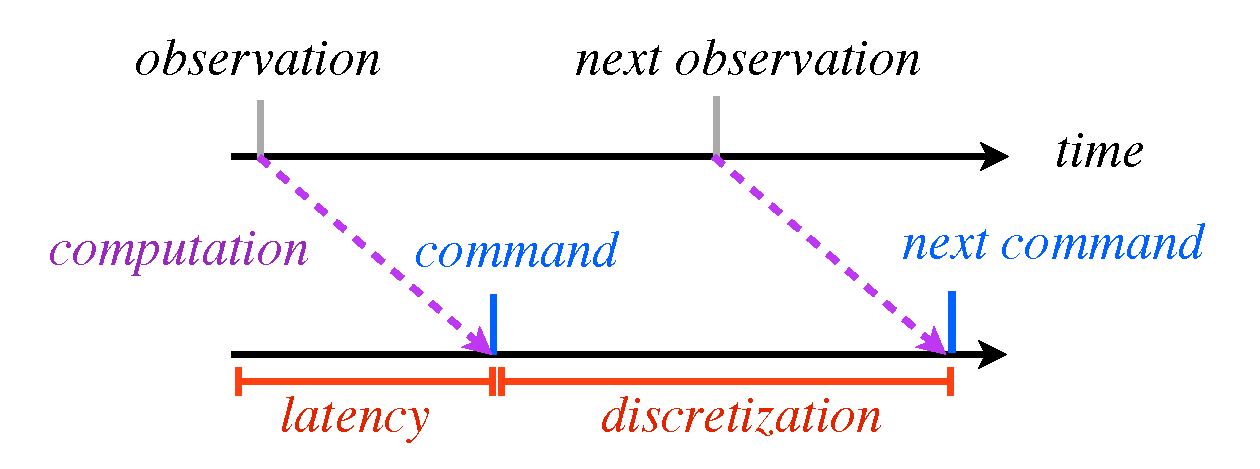
\includegraphics[width=7cm]{figures/slides/latency1}
\par\end{centering}

}
\par\end{centering}

\begin{centering}
\subfloat[Low latency, event-based architecture]{\begin{centering}
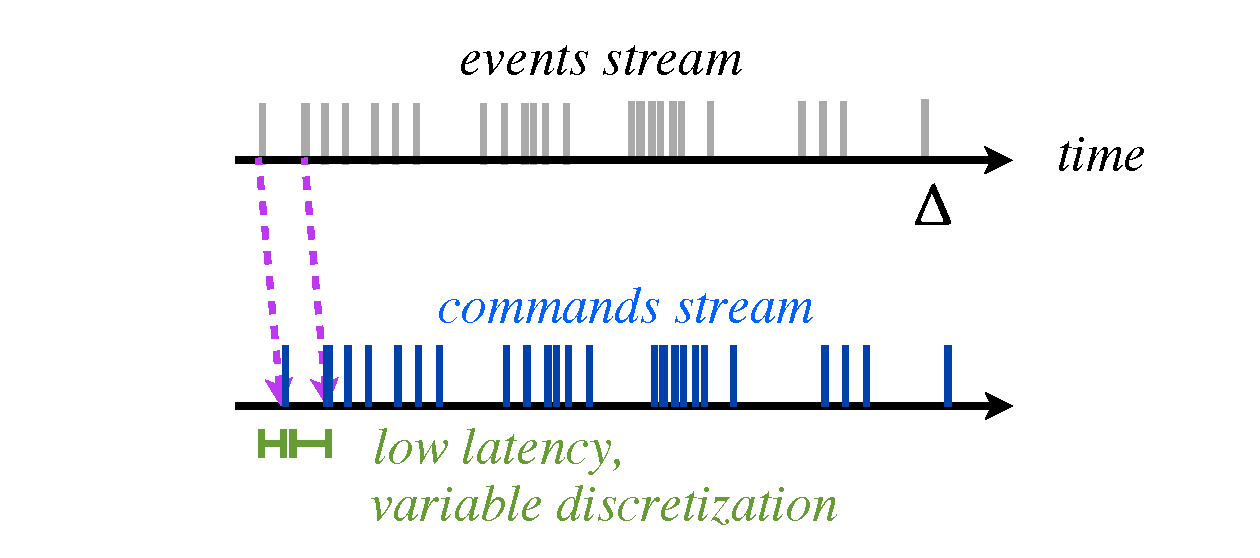
\includegraphics[width=7cm]{figures/slides/latency2}
\par\end{centering}

}
\par\end{centering}

\caption{\label{fig:Discretization-and-latency}To improve the agility of autonomous
flying robots, we need to improve the total latency of the sensing
pipeline. Using a device like a Dynamic Vision Sensor (DVS) we can
theoretically obtain a sensing pipeline which has microsecond latency.}
\end{figure}


The agility of an autonomous flying robot is limited by the speed
of the sensing pipeline. More precisely, ``speed'' can be quantified
in \emph{observations frequency} and \emph{latency} (\prettyref{fig:Discretization-and-latency}).
In current state-of-the art autonomous navigation applications~\cite{Weiss2011}
cameras give observations with frequency of 15--30~Hz and the total
latency, from acquiring the images to processing them, is in the order
of 50--250~ms. To obtain more agile systems, we need to use faster
sensors and low-latency processing.

In this paper, we consider the use of a Dynamic Vision Sensor (DVS)
for pose tracking. The main difference between a DVS and a normal
CMOS camera is that the DVS output is a stream of \emph{events} that
encode \emph{changes} in the brightness. Each event encodes the location
of the change, whether there was a positive or negative change in
brightness, and has a 1~$\mu$s timestamp.  These events are not
unlike spikes in a biological visual system; however, while retinal
ganglion cells show latencies of around 200~ms, the DVS chip has
a latency of $15\,\mu s$.

Theoretically, using a DVS we could obtain sensing pipelines with
a negligible latency compared to dynamics of the platform. We are
a few years to the goal, however. On the hardware side, the DVS camera,
though currently available commercially, has a few limitations, such
as the limited resolution ($128\times128$ pixels), which  will
be increased in the next generation of prototypes currently in development.
On the software side, to take full advantage of this data we need
to rethink completely the way we design robotic sensing pipelines.
It is possible to integrate the events of a DVS camera to simulate
a regular CMOS frame, on which to do standard image processing, however,
that is not desirable, because that would give the same latency of
a regular camera. Ideally, to have the lowest latency for the sensing
pipeline, one would want each single event to be be reflected in a
small but instantaneous change in the commands given to the actuators.
Therefore, we consider approaches that possibly use the information
contained in each single event.

In this paper, we consider the application of pose tracking based
on Active LED Markers (\ALMs), which are infrared LEDs blinking at
 high frequency ($>1\,\mbox{kHz}$). The DVS is fast enough to be
able to distinguish different blinking frequencies, so that we can
also uniquely assign an observable identity to each marker. We envision
that this system could be used for inter-robot localization for high-speed
acrobatic maneuvers, or that, in applications such as rescue robotics,
these markers could be left in the environment to facilitate cooperative
mapping.

One approach to using the DVS data is to cluster the events in order
to find spatio-temporal features, like points or lines, that are then
tracked through time~\cite{delbruck07fast,conradt09pencil,Matthias}.
This approach works well when the camera is static, because the output
is spatiotemporally sparse. 

The algorithm presented in this paper uses a different approach. We
found out that mounting a DVS camera on a flying robot creates a new
set of challenges. Because of the apparent motion of the environment,
the events are not spatiotemporally sparse anymore. Moreover, while
in controlled conditions the DVS camera parameters can be tuned to
obtain the best performance, a robot must be able to work in a wider
range of environmental conditions and be robust to interferences.
To achieve this robustness we have developed an approach that sacrifices
some latency to be more robust to noise and unmodeled phenomena. We
accumulate the events perceived in thin slices of times corresponding
to the blinking frequency ($1$~ms slice for 1~kHz data). This allows
to do detection of the \ALMs position in image space. On top of this,
we use a particle filter for tracking the position in image space
of each detection, and a disambiguation stage to obtain coherent hypotheses
on the joint position of the markers. Finally, we reconstruct the
pose using a standard approach to rigid reconstruction.

We evaluate our method in tracking the pose of a drone during an aggressive
maneuver (a flip). We compare our methods with a traditional approach,
using a CMOS camera and a feature-based visual odometry method. We
verify that our method, with a latency of $1$~ms, is able to reacquire
tracking instantaneously regardless of the fast motion, while the
CMOS data is corrupted by motion blur. We evaluate the reconstruction
accuracy using an OptiTrack system and find values that are compatible
with the low spatial resolution (128$\times$128) of the DVS, which
proves to be the current limitation of this approach.



Software, datasets, and videos illustrating the method are available
at the website \myurl.



\section{The Dynamic Vision Sensor (DVS)\label{sec:The-DVS-camera}}

A regular CMOS camera records a visual scene by taking a stroboscopic
series of still frames. Computer vision and robot perception methods
work on the analysis of each frame separately. This established approach
has some fundamental drawbacks: each pixel gets sampled and processed
over and over again at each frame, independently of its relevance
to the decision to be taken, or whether its value changed. Much processing
power is used for considering redundant information, which translate
into high latencies and low frame rates. In contrast to this, we observe
that in biological systems there is redundancy suppression already
on the \textquotedblleft{}sensor\textquotedblright{}: as recordings
of nerve cells coming from the eye show, the retina mostly responds
to \emph{changes} in the perceived brightness.

The field of\emph{ neuromorphic engineering} tries to reproduce the
main characteristics of the computations done by nervous systems as
VLSI circuits. The computation is \emph{analogic}: currents, voltages
and charges are used for computing, rather than binary representations.
The resulting circuits are also \emph{asynchronous}: like nervous
cells, they operate independently of an external clock for state transitions.
There has been a large amount of research in neuromorphic sensory
systems of different scale and complexity~\cite{liu10neuromorphic}.
The first system to be commercially available is the so-called ``silicon
retina'' or Dynamic Vision Sensor\emph{ }(DVS)~\cite{lichtsteiner08asynchronous}.

Each pixel in the DVS operates independently and asynchronously from
the others. The photons that reach a photodiod produce a photocurrent,
which is converted into a voltage. This voltage gets continuously
compared to the last sampled voltage. As soon as the difference between
these two voltages is larger than a certain threshold, the pixel requests
to send an \emph{event} off chip. After the address and the timestamp
of this event has been registered from a CPLD at the chip periphery,
the pixel is reset, and the most recent voltage gets sampled to be
compared against successive voltages. All of this computation is done
without digitizing the signal. 

Each event carriers the following information: a timestamp, which
has a 1~\textmu{}s resolution, the \emph{address }of the pixel that
observed the change (equivalent to its~$x,y$ coordinates), and the
\emph{polarity} of the change (\pP or \pN). The polarity depends
on the sign of the difference. \pP~events indicate that the brightness
increased, while \pN~events indicated that it decreased.

The parameters that modulate the pixel behavior are dynamically programmed
using a set of bias currents. Some of the parameters that can be dynamically
changed are the temporal contrast frequency cutoff, the \pP \& \pN
threshold, and the event frequency cutoff. 

The sensor therefore only produces output if the observed scene changes.
This is not only the case if the intensity of a light source gets
modulated (as with a blinking LED), but also if a static scene moves
relative to the sensor. If the sensor itself is moved it perceives
all the edges and contours in its visual field.

Sensing the world with a set of autonomous, change-sensitive pixels
has various advantages compared to traditional image sensors:
\begin{itemize}
\item Since the photocurrent gets converted to a voltage on pixel level,
the brightness measurement does not require a uniform exposure time
for all pixels. This leads to the high dynamic range of 120dB which
is capped by the exposure time in conventional image sensors.
\item By only sensing changes, the sensor performs on-chip data compression.
This does not only make the amount of output data dependent on the
activity in a scene, but it also focuses the processing effort on
the region of interest where it is changing. This focusing allows
to create controllers that have update intervals of down to 125~\textmu{}s~\cite{conradt09pencil}.
\item Redundant information does not occupy the output bus and therefore
relevant information can be signaled very fast. The sensor chip itself
has a latency of 15~\textmu{}s. In practice the main limitation to
the latency of prototype systems is not the DVS, but USB communication.
Round-trip latencies of the whole systems using off-the-shelf computer
architectures are in the order of 3~ms~\cite{delbruck07fast}.
\item The high resolution of the event timestamps can be used to investigate
highly dynamics elements in a scene, such as fast motion or, like
in this paper, blinking LEDs. Moreover, because events are asynchronous,
it is not necessary to commit to use a given sampling frequency like
in a conventional sensors.
\end{itemize}
The main drawbacks of the current generation of DVS are its low resolution
of $128\times128$, and the inability to sample the absolute brightness
levels like a normal camera. The low resolution is due to the prototype
fabrication process used (350~nm) and the fact that each pixel is
associated to a complex circuit carrying on the analog computation.
The absolute brightness levels cannot be accessed because the according
technology was not ready for the first series of sensors. But since
the field of event-based vision sensors is steadily growing~\cite{delbruck10activity},
these limitations will soon be overcome. Some of the latest developments
include higher temporal contrast sensitivity of 1.5\%~\cite{serrano13128}
and higher spatial resolution of~$240\times180$ or~$304\times240$,
accompanied with a readout channel for pictures and movies that simulates
a CMOS camera~\cite{posch11qvga,berner13240}. 

Other ongoing efforts include increasing the availability of the embedded
version of the sensor (eDVS, used in~\cite{conradt09pencil}), which
weighs only a few grams and measures~$30\times50\times50$~mm. Furthermore,
future versions of event based vision sensors are expected to include
a USB 3.0 interface for higher data transmission rates.


\vfill\newpage


\section{Hardware setup and event data\label{sec:Hardware-setup-and}}

This section describes the hardware setup and gives an intuition of
the event data that a DVS produces.


\subsubsection{DVS and its interface\label{sec:interface}}

The DVS attaches to a computer using a common USB port. The camera
is distributed with a portable software framework written in Java
called jAER~\cite{jaer}. This project, developed in C++ for maximum
efficiency, needed a special driver to be developed, based on the
Thesycon USB device driver~\cite{thesycon}. The events are transmitted
from the camera in packets of up to several hundred events; however,
each event is independently tagged at the source with its proper timestamp.



\subsubsection{Active LED Markers (\ALMs)\label{sec:leds}}

The LED controller is based on the bronze board~\cite{bronzeboard}
from iniLabs, which is based on an AVR32.  We used infrared LEDs
since the DVS is very sensitive in the infrared spectrum. 



In our setup we could easily change the PWM frequency to the LEDs.
An upper bound on the detectable frequency depends on the power of
the LEDs and the distance to the camera; a DVS camera is not magic:
there must be a large enough change in the number of photons reaching
the photoreceptor to trigger an event. In our setup we found 2~KHz
to be an adequate number. The frequencies for each LEDs were then
decided in the interval 1--2~KHz making sure we did not choose frequencies
with common harmonics. A reasonable lower bound on the blinking frequency
was found experimentally to be $1$~KHz to minimize the confusion
between with background motion (see \prettyref{sub:Alternate-events-and-motion}
below).


\subsubsection{Statistical properties of event sequences}

\begin{figure}[b]
\begin{centering}
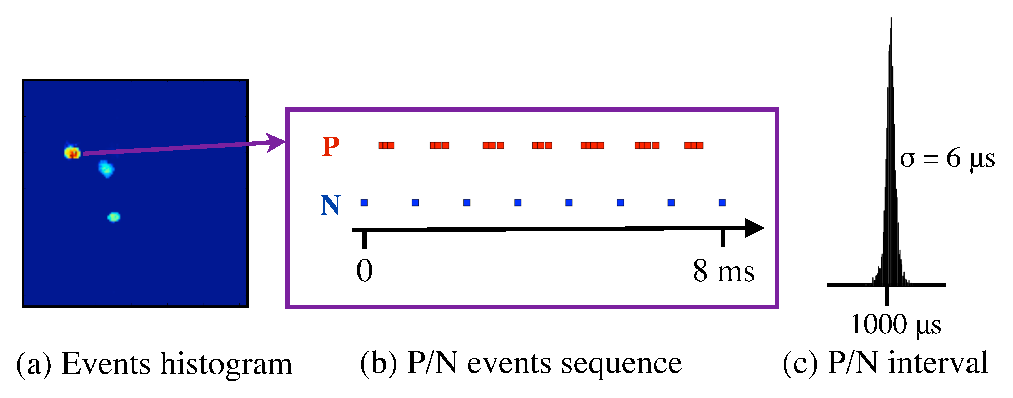
\includegraphics[width=8.6cm]{figures/slides/event_sequence}
\par\end{centering}

\caption{\label{fig:events-hist}Example event sequence from a DVS looking
at an Active LED Marker (\ALM). Subfigure (a) shows the histogram
of events seen from a fixed camera looking at three \ALMs. The difference
in numbers is due to the different frequencies of the \ALMs. Subfigure
(b) shows a slice of the events seen at a particular pixel near the
center of one of the \ALMs which has a blinking frequency of 1 KHz.
The data is a series of events with positive (\pP) and negative (\pN)
events. (c) The sequence of \pPN transitions are highly regular;
in this data we observed that the distribution of the intervals is
well approximated by a Gaussian with mean $1000\,\mu s$ and standard
deviation $\sigma=6\,\mu s$. }
\end{figure}


\prettyref{fig:events-hist} gives an intuition of how the data looks
like. In this scenario both the \ALMs and the DVS are fixed. \prettyref{fig:events-hist}\emph{a}
shows the histogram of the number of events coming from a particular
pixels. The three peaks are the three \ALMs ($f=500,700,1000\,\mbox{Hz}$).
The number of events is different for each peak because the frequencies
differ. The halo in \prettyref{fig:events-hist}\emph{a} cannot be
explained by the refractive properties of the optics, and is probably
due to non-ideal local interactions among neighbors in the sensing
array.

\prettyref{fig:events-hist}\emph{b} shows the sequence of events
obtained from one particular pixel, corresponding to an \ALM  with
a frequency of 1~KHz. There is a different number of P and N events,
which tells us that we cannot really interpret the DVS data as simply
the derivative of the image. 

For this particular data, the P events arrive noisily, while the N
events arrive more regularly. Note that the what we observe here is
the combination of the LED dynamics with the dynamics of the photoreceptor
and the nonlinear detector. Experimentally we found that the interval
between successive P/N transitions is very repeatable: we have observed
that the jitter is well approximated by a Gaussian with standard deviation
equal to $6\,\mu s$ (\prettyref{fig:events-hist}\emph{c}).


\subsubsection{Effect of motion\label{sub:Alternate-events-and-motion}}

\begin{figure}[b]
\centering{}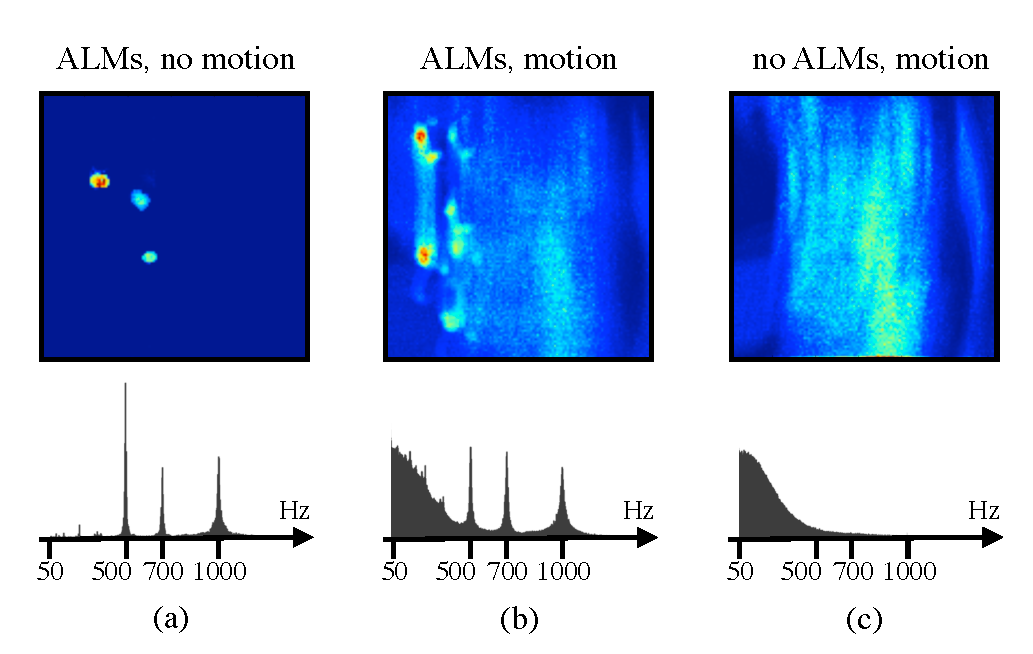
\includegraphics[width=8.6cm]{figures/slides/motion}\caption{\label{fig:switch-hist}Comparison of transition events statistics
in three cases: a)~visible markers, without motion; b)~with camera
motion; c)~with camera motion but no marker visible. Note in (c)
that the motion of the camera creates apparent motion of the environment
and a large number of events; however they are of a low frequency.
In this case, the events from the background are negligible after
$700$~Hz, though this depends on the statistics of the environment
and the speed of the motion. We can choose the frequencies of the
markers high enough such that they are not confused as background
motion.}
\end{figure}


Things get more complicated when the camera is moving, because the
apparent motion of the environment creates changes in luminance that
are unrelated to the \ALMs. However, we have found that we can discriminate
between the two types of events based on their temporal statistics.

\prettyref{fig:switch-hist} shows the histogram of frequencies of
the P/N transitions in three scenarios: a)~a fixed camera looking
at fixed \ALMs; b)~a moving camera looking at fixed \ALMs; c)~a
moving camera with no LEDs. From this data we can see that the motion
of the camera generates a large number of events, but at low frequencies,
and notwithstanding the motion, we can still see very clearly the
peaks originated from the markers. Therefore, if we choose the marker
frequencies high enough, we can filter for the camera motion just
by ignoring the events corresponding to frequencies under a certain
threshold. 


\vfill\newpage

\begin{figure*}
\centering{}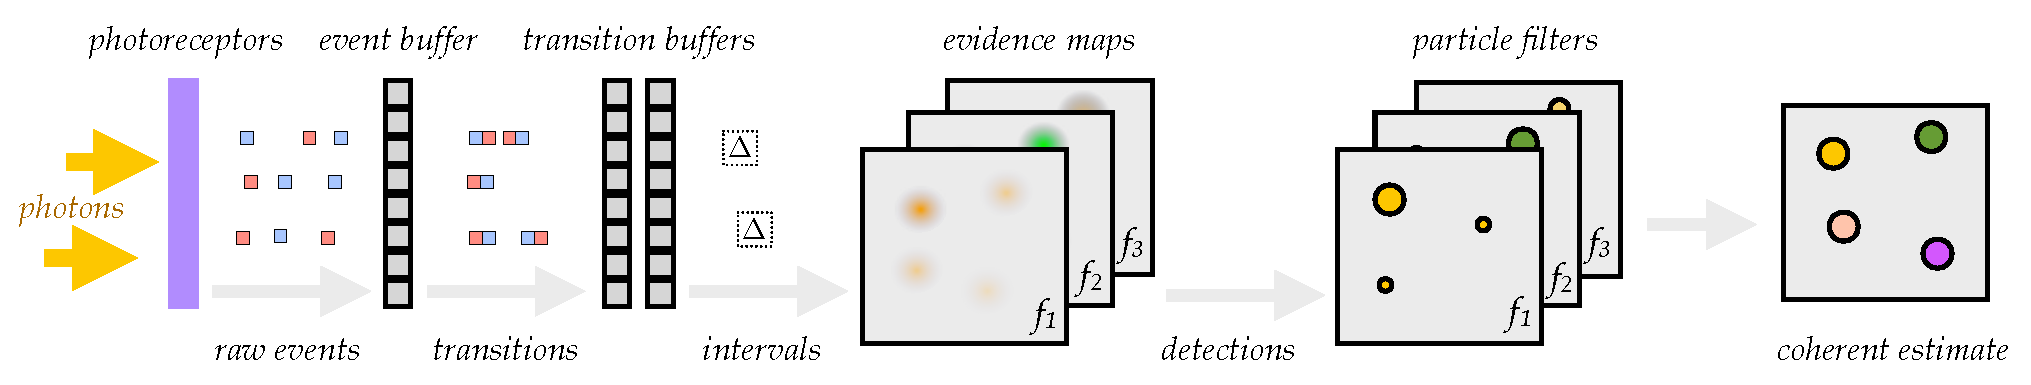
\includegraphics[width=18cm]{figures/slides/overall2}\caption{The first stage of our method consists in buffering the raw events,
which have either \pP or \pN polarity, as to find the transitions,
either \pPN or \pNP. Then, we look at the intervals~$\Delta$ between
two transitions of the same type. These will be converted into votes
in an evidence map tuned to each frequency. From the evidence map
we extract local maxima, which are the instantaneous detections of
where is each \ALM. The rest of the method is standard: for each
frequency we use a particle filter to be robust to missed detections;
then we choose the combination of particles that gives a coherent
global estimate for all \ALMs.}
\end{figure*}


\vfill\pagebreak


\section{DVS-based Active LED Marker tracking }

This section describes our method for tracking the position of a set
of \ALMs from the output of a DVS. The input to the algorithm is
a sequence of events representing the change of luminance in a single
pixel. The output is an estimate of the pose of the quadrotor. We
describe the algorithm as a sequence of stages that process asynchronous
events; in principle, several of them could be implemented in hardware.

\begin{figure}[H]
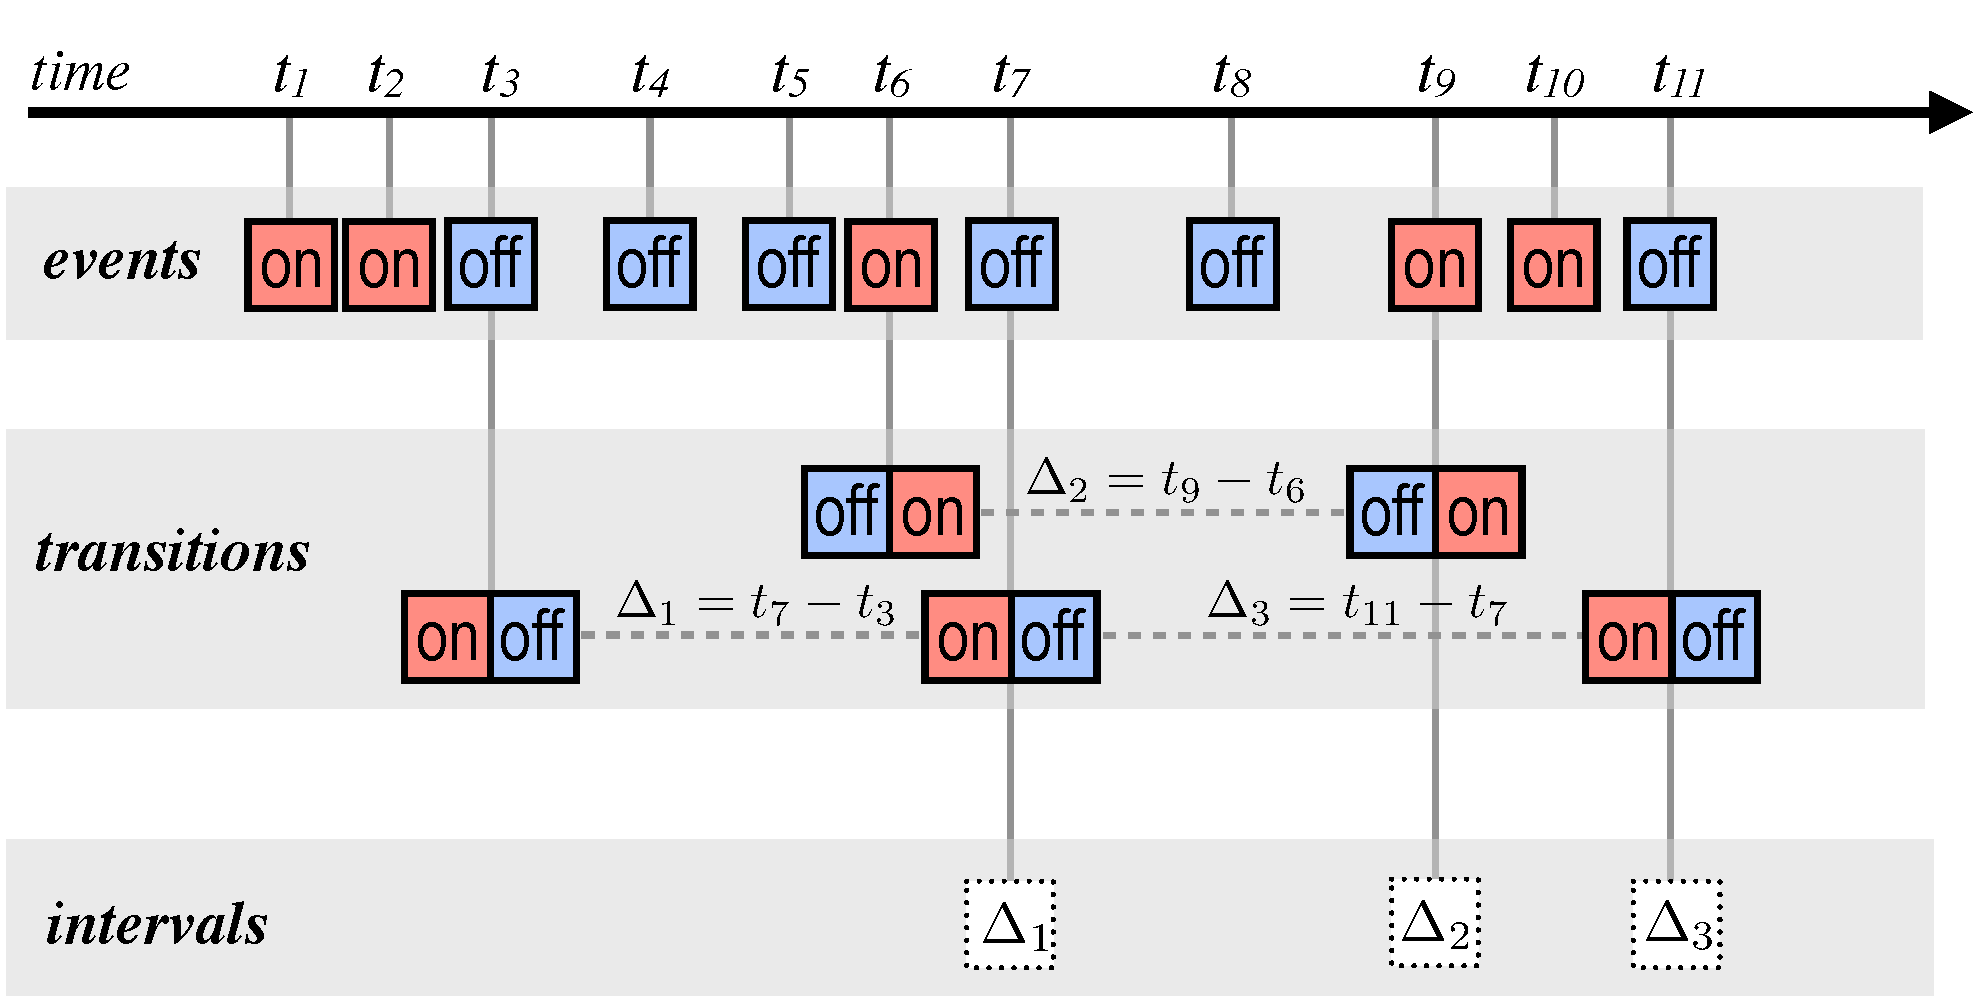
\includegraphics[width=8.6cm]{figures/slides/stages3}

\caption{\label{fig:A-single-pixel}A single pixel produces an irregular series
of raw events, each consisting of a timestamp, a location, and a polarity,
either \pP or \pN polarity. The first stage of processing consists
in extracting the \pPN or \pNP transitions. The second stage consists
at looking at two successive transitions of the same kind. For example,
in this figure, two successive \pPN transitions at time~$t_{3}$
and~$t_{7}$ generate a hyper-transition with interval $\Delta=t_{7}-t_{3}$.
Assuming that these events are generated by a blinking \ALM, the
value of~$\Delta$ is a good robust estimator of the blinking period.}
\end{figure}



\subsection{Raw events}

The input to the algorithm is the sequence of generated events. We
use $k$ to index the events. Each event can be represented by a tuple
\[
\langle t_{k},\: p_{k},\:\langle x_{k},y_{k}\rangle\rangle,
\]
where: 
\begin{itemize}
\item The scalar $t_{k}$ is the timestamp of the event. Timestamps are
not equispaced in time, as events are asynchronously generated by
each pixel.
\item The value $p_{k}\in\{\pP,\pN\}$ is the \emph{polarity}. The \pP
polarity implies a positive change in brightness, while the \pN polarity
a negative change. This value can be interpreted as the sign of the
instantaneous brightness change.
\item The coordinates $\left\langle x_{k},y_{k}\right\rangle $ identify
the pixel that triggered the event.
\end{itemize}

\subsection{Transitions}

The first stage of our algorithms transforms the sequence of the raw
$\{\pP,\pN\}$ events into a sequences of \emph{transition events}
$\{\pPN,\pNP\}$. This is done independently for each pixel. Consider
the events that are produced by a given pixel at coordinates~$\left\langle x,y\right\rangle $
and let~$k$ be the sequence index for the events of that pixel only.

At all times, we remember the last event timestamp~$t_{k-1}$ and
its polarity~$p_{k-1}\in\{\pP,\pN\}$. Every time the polarity of
the current event~$p_{k}$ is different than the previous polarity~$p_{k-1}$,
we create a \emph{transition event}. If the polarity is the same,
no transition event is generated. This is described by the rules in
\prettyref{tab:From-raw-events}. 

A transition event is a tuple 
\[
\langle t_{k},\: q_{k},\:\langle x_{k},y_{k}\rangle\rangle,
\]
where: 
\begin{itemize}
\item The scalar $t_{k}$ is the timestamp of the \emph{second} event that
triggered the transition.
\item The value $q_{k}\in\{\pP,\pN\}$ is the transition polarity, which
is either positive-to-negative~(\pPN) or negative-to-positive~(\pNP).
\item $\left\langle x_{k},y_{k}\right\rangle $ are the pixel coordinates.
\end{itemize}
\begin{center}
\begin{table}[b]
\begin{centering}
\caption{\label{tab:From-raw-events}From raw events to transitions}

\par\end{centering}

\centering{}\normalsize %
\begin{tabular}{ccc}
\emph{last event} & \emph{current event} & \emph{transition event}\tabularnewline
\hline 
\multirow{2}{*}{$\langle t_{k-1},\ \pP,\:\langle x,y\rangle\rangle$} & $\langle t_{k},\ \pP,\:\langle x,y\rangle\rangle$ & none\tabularnewline
 & $\langle t_{k},\ \pN,\:\langle x,y\rangle\rangle$ & $\langle t_{k},\ \pPN,\:\langle x,y\rangle\rangle$\tabularnewline
\multirow{2}{*}{$\langle t_{k-1},\ \pN,\:\langle x,y\rangle\rangle$} & $\langle t_{k},\ \pP,\:\langle x,y\rangle\rangle$ & $\langle t_{k},\ \pNP,\:\langle x,y\rangle\rangle$\tabularnewline
 & $\langle t_{k},\ \pN,\:\langle x,y\rangle\rangle$ & none\tabularnewline
\end{tabular}
\end{table}

\par\end{center}


\subsection{Hyper-transitions}

The next stage of processing looks at the interval between successive
transitions of the same type. For each pixel, we remember the last
transition of either type (\pPN or \pNP) in a separate storage;
then, for each transition, we generate a ``hyper-transition'', which
is a tuple of the kind 
\[
\langle t_{k},\,\Delta_{k},\:\langle x_{k},y_{k}\rangle\rangle,
\]
where~$\Delta_{k}$ is the interval between transitions of the same
kind, and~$\langle x_{k},y_{k}\rangle$ are the coordinates (\prettyref{fig:A-single-pixel}).
Note that we dropped the polarity of the transitions, as they are
not needed in the following stages.


\subsection{Evidence maps}

We suppose to have been given a set of~$n$ frequencies~$\{f_{i}\}$,
$i\in\{1,n\}$ corresponding to the~$n$ \ALMs to track. For each
frequency separately we construct an ``evidence map'' $I_{i}(\left\langle x,y\right\rangle ,t)$
over the visual field corresponding to the probability that the \ALM
is at that pixel. Each hyper-transition contributes to all evidence
maps, but with a different weight, so that we can integrate all information
and do not commit to assigning an event to a given frequency. This
approach is robust to noisy data and background motion. For non-noisy
data, an alternative approach that uses clustering of events works
just as well~\cite{Matthias}.

A hyper-transition with interval $\Delta_{k}$ contributes to the
evidence map of frequency~$f_{i}$ with a weight that is proportional
to~$p(\Delta_{k}\mid f_{i})$; that is, the likelihood that a marker
\ALM with that frequency produces a hyper-transition of that interval.
The distribution $p(\Delta_{k}\mid f_{i})$ is found experimentally
to be well approximated by a Gaussian, as seen in the data in \prettyref{fig:switch-hist}\emph{b}:
\begin{equation}
p(\Delta_{k}\mid f_{i})=\mathcal{N}\left(\frac{1}{\Delta_{k}}-f_{i},\sigma^{2}\right).\label{eq:lik_delta}
\end{equation}
In our experimental setting, the standard deviation is approximately~$\sigma=30\ \mbox{Hz}$.
The evidence maps collect events within a time slice corresponding
to an interval of~$1/f_{i}$. Therefore, the value of the evidence
map $I_{i}(\left\langle x,y\right\rangle ,t)$ for a pixel~$x,y$
and at time~$t$ is given by the sum of the contributions of all
events at the given pixel and in the interval~$\left[t-1/f_{i},t\right]$:
\[
I_{i}(\left\langle x,y\right\rangle ,t)=\sum_{t_{k}\in\left[t-\frac{1}{f_{i}},t\right]\wedge\left\langle x_{k},y_{k}\right\rangle =\left\langle x,y\right\rangle }\mathcal{N}\left(\frac{1}{\Delta_{k}}-f_{i},\sigma^{2}\right).
\]
To increase robustness at the expense of latency, it is also possible
to use multiples of~$1/f_{i}$ as the time slice interval.

At the end of the time slice, the evidence map~$I_{i}(\left\langle x,y\right\rangle ,t)$
can be interpreted as the likelihood that the $i$-th \ALM with frequency~$f_{i}$
is at position~$\left\langle x,y\right\rangle $. In our experimental
setting, this map is multimodal, with a strong peak at the true position
of the marker, and lower peaks at the positions at the other markers,
because each event contributes weakly, according to~\prettyref{eq:lik_delta},
also to the evidence maps of the other frequencies. 

We extract~$m$ local maxima, at least~$\delta$ pixels from each
other (in our experiments $m=3$, $\delta=15\,\mbox{px}$). The value
of the evidence map at the local maxima is used as a weight~$w$
to be carried forward to the next stage. The detections generated
in this way have a time~$t$, coordinates~$\left\langle x,y\right\rangle $
and the weight~$w_{j}^{i}$:
\[
\{\langle t,\,\langle x_{j}^{i},y_{j}^{i}\rangle,\, w_{j}^{i}\rangle\},\ j\in\{1,\dots,m\}.
\]



\subsection{Filtering and reconstruction}

Once we have these detections, the method proceeds in a conventional
way, as in any tracking problem, to achieve robustness to missed detections
and false alarms. 

First we use a particle filter to evolve particles for each frequency.
Each particle has coordinates $\langle x,y\rangle$, a weight~$w$
(carried over from the last step), as well as an isotropic spatial
uncertainty~$r$, which starts at $1\,\mbox{px}$. The uncertainty
grows using a motion model, which should be chosen according to how
on how fast things are predicted to move on the visual field. We have
computed that for the range of motions of a quadrotor, in our experimental
setting the maximum apparent motion is approximately $1$ pixel/ms.

There is a particle filter for each frequency. The particles in each
filter represent the posterior over the pose of one \ALM. To look
for a globally consistent solution, we choose the combination of particles
from all filters with the highest combined weight such that no two
markers can be too close to each other (in our experiments, $d=15$
pixels). Assuming we have the position of the \ALMs in image space,
and we know the relative position of the markers in the world, we
can reconstruct the pose of the object using established techniques
for rigid reconstruction.



\section{Experiments\label{sec:experiments}}

The experiments consider the advantages of a DVS-based tracking solution
with respect to a tracking solution based on a traditional CMOS camera.
We compare the DVS-based \ALM tracking with vision-based tracking
using the PTAM algorithm, using the output of an OptiTrack system
as the ground truth. The data show that the DVS-based tracking is
able to deal with faster motions due to the minimal latency, but the
precision of the reconstructed pose is limited by the low resolution
of the sensor.



\begin{figure}[b]
\centering{}\hfill{}\subfloat[\label{fig:quadcopter_belly}\ALMs configuration]{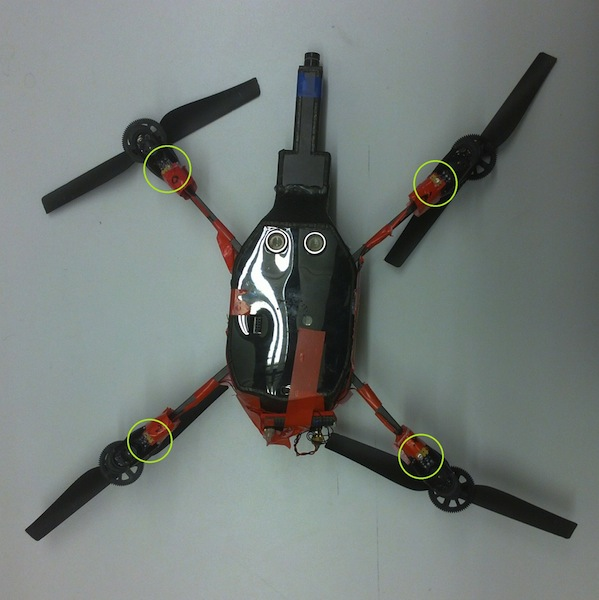
\includegraphics[height=3.5cm]{figures/quadcopter_belly_small} }\hfill{}\subfloat[\label{fig:Infrared-markers-used}Infrared markers]{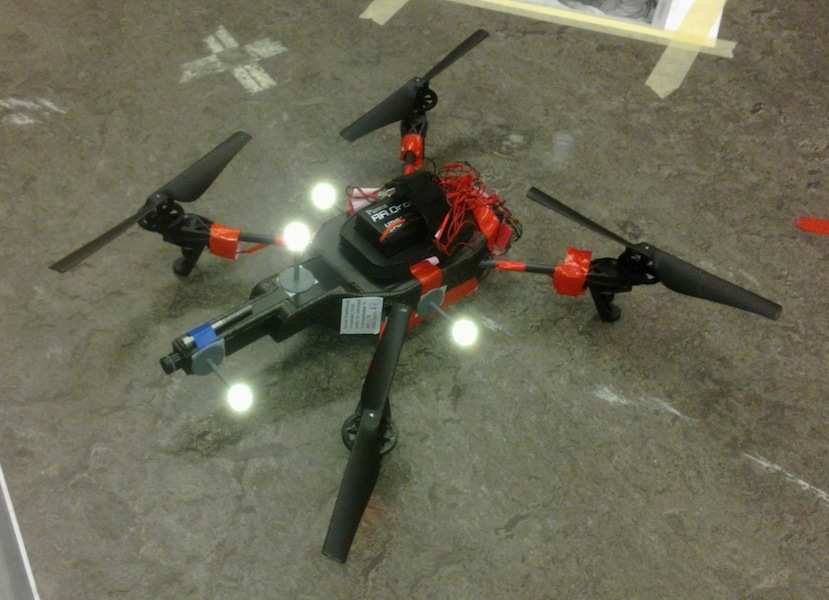
\includegraphics[height=3.5cm]{figures/marked_quadrotor_small}

}\hfill{} \caption{\label{fig:marked_quadrotor}The ARDrone 2.0 equipped with four \ALMs
(shown in \emph{a}) tracked by the DVS, and reflective markers used
by the OptiTrack (shown in \emph{b}). }
\end{figure}



\subsection{Hardware}


\subsubsection{Robot platform}

We used the commercially available ARDrone 2.0 We attached four custom-built
\ALMs to the bottom of the platform (\prettyref{fig:quadcopter_belly}).
Each LED was fixed facing downwards, one under each of the four rotors,
so that the four were lying on a plane forming a square of 20cm side
length. The USB connector available on the drone provided power to
the microcontroller and \ALMs. The drone has also a front-facing
$720\times980$ CMOS camera that is used in these experiments, while
the ground-facing camera is not used.


\subsubsection{DVS}

The DVS128 camera was used for the tests. This model is currently
commercially available from INI labs. It has a resolution of $128\times128$
pixels. The lens attached gave the sensor a FOV of approximately 65\textdegree{},
giving a resolution of 0.5~pixels/\textdegree{}. For tracking the
quadcopter, the DVS was installed on the floor facing upwards. Note
that the relative motion between DVS and quadcopter would be the same
if the \ALMs were on the floor and the DVS on board.


\subsubsection{OptiTrack}

To measure the pose estimation accuracy we used a OptiTrack tracking
system from NaturalPoint~\cite{optitrack}, which is a marker-based
optical motion tracking system using active infrared light and reflective
marker balls. Four markers have been applied to the drone (\prettyref{fig:Infrared-markers-used}).
Our lab setup comprised 10 cameras in a $6\times8\,\mbox{m}$ area;
the cost of this system is approximately 20,000~CHF (\$21,000). The
sampling frequency used was $250$~Hz. The accuracy is stated as~$\sim1$~mm
by the manufacturer, but this seems an optimistic estimate based on
our experience with the system.



\begin{figure*}
\begin{centering}

\par\end{centering}

\begin{centering}
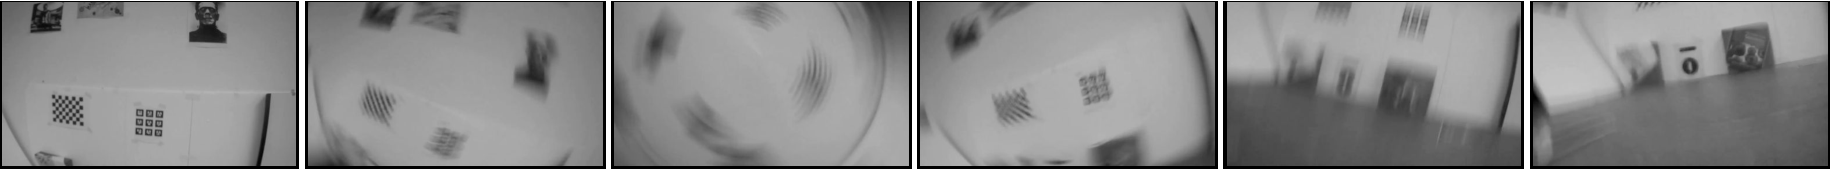
\includegraphics[width=17cm]{figures/slides/flip_sequence_small}
\par\end{centering}

\caption{\label{fig:Motion-blur-induced}Motion blur induced on CMOS image
from flip motion.}
\end{figure*}



\subsubsection{Motion}

The prototypical aggressive maneuver that we use is a ``flip'' of
the quadcopter, i.e. a $360^{\circ}$ roll. During the flip the frontal
camera images are severely blurred (\prettyref{fig:Motion-blur-induced}). 




\subsubsection{Interference OptiTrack / DVS}

We encountered an unexpected incompatibility between OptiTrack and
DVS. The OptiTrack uses high-power infrared spotlights. In the OptiTrack's
standard configuration, the spotlights are pulsed at a high frequency.
This is of course invisible to normal sensors and to the human eye,
but it was a spectacular interference for the DVS. Like most cameras,
the DVS is most sensitive in the infrared spectrum and is much faster
than the OptiTrack strobing frequency. This generated a buffer overflow
on the DVS as the electronics could not handle the large number of
events to be processed contemporaneously. Eventually we understood
how to deactivate the strobing for all the cameras prior to recording.
Still there was a slight residual interference by the infrared illumination
from the OptiTrack, but it should have relatively little impact to
the results of our experiments.


\subsection{Methods}

We compare three ways to track the pose of the quadcopter: 1)~The
output of our DVS-based \ALM tracking method; 2)~The OptiTrack output;
3)~The output of a traditional feature-based tracker using the data
from the conventional CMOS camera mounted front-facing on the drone.
The image data was streamed to a computer via network interface, were
the parallel tracking and mapping algorithm (PTAM)~\cite{PTAM} was
employed for pose estimation.


\subsubsection{Data recording, synchronization, and alignment\label{sec:datarecording}}

Using this setup we did several recordings, in which we recorded the
OptiTrack tracking data, using its native format, the image data using
a ROS interface, as well as the raw event data from the DVS in the
native format. 

To synchronize the data from different sources we used a motion induced
cue. We moved manually the drone up and down, generating an approximated
sinusoid curve in the position data, which allowed easy manual matching
of the sequences.

After adjusting for the delay, the data sets were brought to the same
number of samples with a common time stamps. As our algorithm's output
has a lower sampling rate than the OptiTrack (1~KHz vs 250~Hz),
the OptiTrack data was resampled by linear interpolation.



As a final step, the time series were put in the same frame of reference.
Given two sequences of points~$\boldsymbol{x}_{k},\boldsymbol{y}_{k}\in\mathbb{R}^{3}$,
the rototranslation $\left\langle \boldsymbol{R},\boldsymbol{t}\right\rangle \in\mathsf{SE}(3)$
that matches them can be found by solving the optimization problem

\begin{equation}
\begin{aligned}\min_{\left\langle \boldsymbol{R},\boldsymbol{t}\right\rangle \in\mathsf{SE}(3)}\sum_{k}\|\boldsymbol{x}_{k}-(\boldsymbol{R}\boldsymbol{y}_{k}+\boldsymbol{t})\|^{2},\end{aligned}
\label{eq:leastsquares}
\end{equation}
which is a classic Procrustes problem~\cite{gower04procrustes}.




\subsection{Results \label{sec:evaluation}}

We recorded data from 18 flips, of which only 6 were successful. During
the recordings we met a number of unforeseen difficulties due to our
modifications to the drone. Having attached the LEDs and microcontroller
to the drone we found that it had become unstable during flight and
hard to control due to the additional weight, so while it could hover
normally, it did not have enough thrust to stabilize itself after
a flip.




\subsubsection{Tracking downtimes\label{sec:trackingspeed}}

During a flip, both the DVS and PTAM lose tracking: PTAM loses tracking
while the image is blurred; the DVS loses track when the \ALMs are
not visible from the ground. The comparison of these ``blackout times''
gives a direct measurement of the latency of the two systems. 



The length of a flip was measured by considering the roll data from
the OptiTrack, taking the interval between the last measurement before
the flip and the first measurement after the flip when the helicopter
was in a level orientation to the floor. 

To measure the onset and offset of the blackout for the DVS, we considered
the last sample before losing track (i.e. where the interval position
samples were considerably higher than the mean sampling rate) and
the first sample of reacquiring track (regaining a steady sample rate).
The equivalent operation was performed on the PTAM data. 



Table \ref{tab:downtime_tab} shows the mean standard deviation of
the different approaches. Our algorithm lost track during the average
time of 0.35 seconds. PTAM lost track for a mean of 0.8 seconds, which
is more than twice the time of the DVS and takes longer than the average
duration of a flip. One can clearly see that the time where tracking
is lost is much shorter with our approach in respect to PTAM. The
results emphasize that the DVS is faster in recovering lost tracks
than the PTAM approach due to not suffering from motion blur. As verified
with our recordings, the downtimes of the DVS correspond to losing
sight of the LED markers because of their emission angle. With a suitable
configuration of either more markers or dynamic vision sensors, tracking
could be maintained during the whole flip. 

\begin{table}
\caption{\label{tab:downtime_tab} Tracking downtime intervals and the flip
duration.}
\vspace{-2mm}\centering%
\begin{tabular}{r|l}
\rule{0pt}{1em}DVS  & $0.35\pm0.10$ s\tabularnewline
PTAM  & $0.80\pm0.33$ s\tabularnewline
flip duration & $0.56\pm0.15$ s\tabularnewline
\end{tabular}\vspace{-2mm}
\end{table}







\subsubsection{Accuracy of estimated pose\label{sec:poseestimationeval}}

The statistics of the estimation error for DVS and PTAM, considering
the OptiTrack as the ground truth, are summarized in \prettyref{tab:Estimation-error}
and shown in graphical form in~\prettyref{fig:errors}.

As for the translation, the DVS estimation error is roughly two times
lower than PTAM (\prettyref{fig:errors}\emph{a}). Although the spread
of outliers is higher in our approach compared to PTAM, the translation
errors of the latter technique show a broader distribution around
their median. Overall this proves that the DVS approach has higher
accuracy with less spread, if we neglect the extreme tails of the
distribution.

\prettyref{fig:errors}\emph{b}--\emph{d} show the error distribution
for roll, pitch and yaw respectively. The DVS performs worse in roll
and pitch compared to yaw. This was to be expected, because of the
position of the \ALMs. As roll and pitch play a minor roll in quadrotor
pose estimation these can be neglected for finding the drone's orientation.
The DVS performs slightly worse than PTAM with a mean error of 6\textdegree{}
and a deviation of 15\textdegree{} (\prettyref{tab:Estimation-error}).
This is explained by the much lower resolution of the DVS ($128\times128$
pixels) compared to the CMOS camera used by PTAM ($720\times980$
pixels). 

\begin{table}[H]
\caption{\label{tab:Estimation-error}Estimation error of DVS and PTAM compared
to Optitrack}


\centering

\newcommand{\tmean}{mean\xspace}
\newcommand{\incm}{[cm]}
\newcommand{\indeg}{[$^\circ$]}
\newcommand{\tstd}{std.dev.\xspace}
\renewcommand{\tabcolsep}{3pt}
\footnotesize

\begin{tabular}{r|rl|rl|rl|rl}
\multicolumn{1}{r}{} & \multicolumn{2}{c}{(a) Translation} & \multicolumn{2}{c}{(b) Roll } & \multicolumn{2}{c}{(c) Pitch} & \multicolumn{2}{c}{(d) Yaw}\tabularnewline
\cline{2-9} 
DVS\rule{0pt}{1em} & 8.9  & $\pm$ 12.6 cm  & 19  & $\pm$ 27\textdegree{} & 17  & $\pm$ 18\textdegree{}  & 6  & $\pm$ 15\textdegree{}\tabularnewline
PTAM & 19.0 & $\pm$ 12.4 cm & 7  & $\pm$ 22\textdegree{} & 5  & $\pm$ 11\textdegree{}  & 3  & $\pm$ 10\textdegree{}\tabularnewline
\end{tabular}

\end{table}


\begin{figure*}
\begin{centering}
\vspace{-2mm}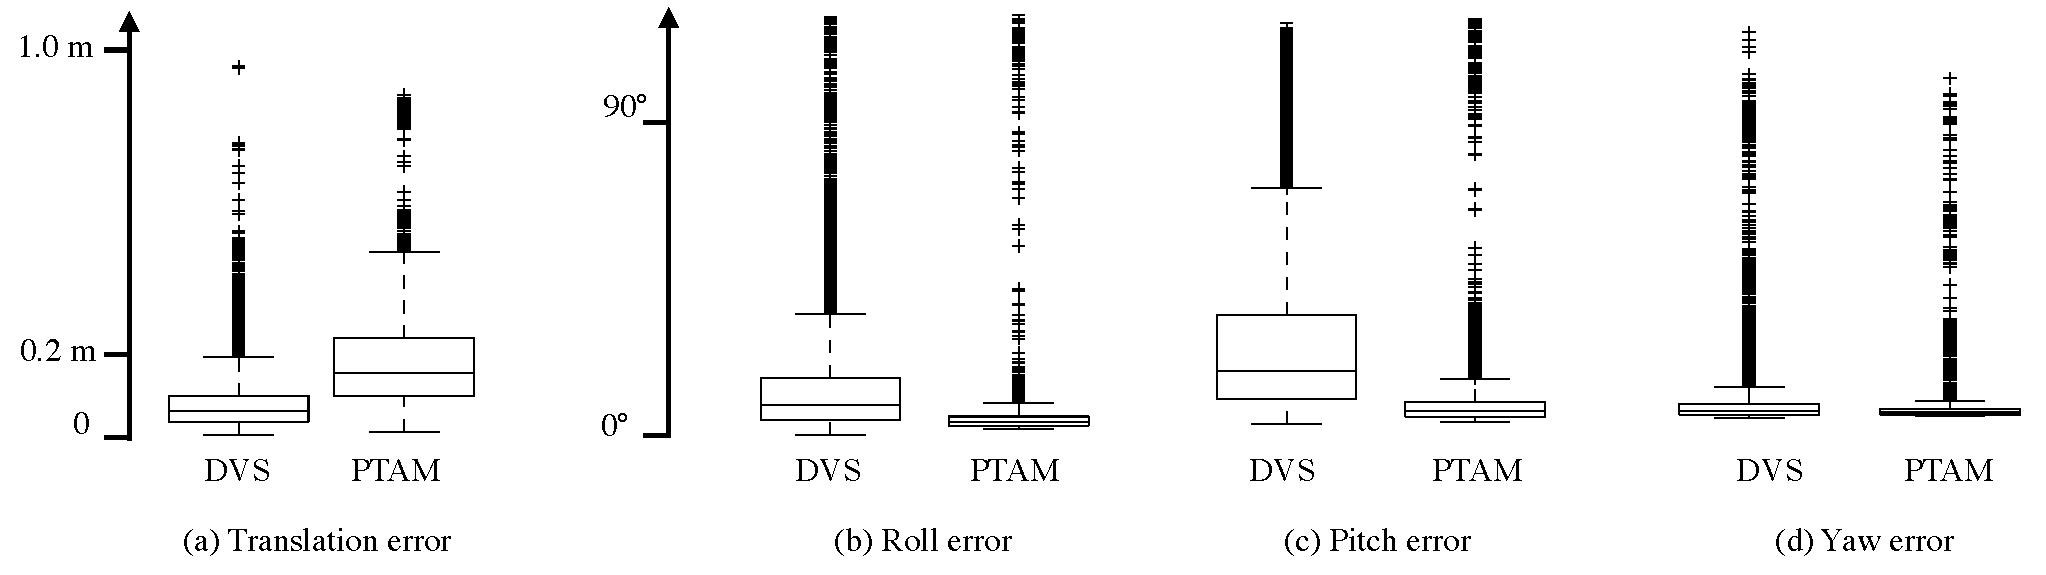
\includegraphics[width=17.5cm]{figures/slides/errors}\vspace{-4mm}
\par\end{centering}

\caption{\label{fig:errors}Distributions of the errors of DVS/PTAM in reference
to the OptiTrack measurements. The data is synthesized in~\prettyref{tab:Estimation-error}.}
\end{figure*}






\section{Conclusions\label{sec:conclusion}}

Fast robots need fast sensors. A dynamical vision sensor (DVS) returns
changes in the visual field with a latency in the microsecond resolution.
This technology is the most promising candidate for enabling highly
aggressive autonomous maneuvers for flying robots. The current prototypes
suffer a few limitations, such as a relatively low resolution, and
a large weight that cannot be put onboard an agile drone. However,
these problems will be resolved in a few years. In the mean time,
the sensing pipeline must be completely re-designed to take advantage
of the low latency.

This paper has presented the first pose tracking application using
DVS data. We have shown that the DVS can detect Active LEDs Markers
(\ALMs) and disambiguate their identity if different blinking frequencies
are used, thus thus avoiding the complexity of data association. The
algorithm that the we developed uses a Bayesian framework, in which
we accumulate evidence of every single event into ``evidence maps''
that are tuned to a particular frequency. The temporal interval can
be tuned and it is a tradeoff between latency and precision. In our
experimental conditions it was possible to have a latency of only
1~ms. After detection, we used a particle filter and a multi-hypothesis
tracker. 

We have evaluated the use of this technology for tracking the motion
of a quadrotor during an aggressive maneuver. Experiments show that
the DVS is able to reacquire stable tracking with negligible delay
as soon as the LEDs are visible again, without suffering from motion
blur, which limits the traditional CMOS-based conventional feature
tracking solution. However, the precision in reconstructing the pose
is limited because of the low $128\times128$ resolution. Future work
involving the hardware include improving the \ALMs by increasing
their power and their angular emittance field, as we have found these
to be the main limitations.

In conclusion, DVS-based \ALM tracking promises to be a feasible
technology that can be used for fast tracking in robotics.







\textbf{Acknowledgements}: We gratefully acknowledge the contribution
of Christian Saner for \xxx, of Yves \xxx as our pilot, and Matia
Pizzoli for the CMOS-based tracking experiments.


\vfill\newpage

\printbibliography



\cleardoublepage

\end{document}
